%%%%%%%%%%%%%%%%%%%%%%%%%%%%%%%%%%%%%%%%%
% Beamer Presentation
% LaTeX Template
% Version 1.0 (10/11/12)
%
% This template has been downloaded from:
% http://www.LaTeXTemplates.com
%
% License:
% CC BY-NC-SA 3.0 (http://creativecommons.org/licenses/by-nc-sa/3.0/)
%
%%%%%%%%%%%%%%%%%%%%%%%%%%%%%%%%%%%%%%%%%

%----------------------------------------------------------------------------------------
%	PACKAGES AND THEMES
%----------------------------------------------------------------------------------------

\documentclass{beamer}

\mode<presentation> {

% The Beamer class comes with a number of default slide themes
% which change the colors and layouts of slides. Below this is a list
% of all the themes, uncomment each in turn to see what they look like.

%\usetheme{default}
%\usetheme{AnnArbor}
%\usetheme{Antibes}
%\usetheme{Bergen}
%\usetheme{Berkeley}
%\usetheme{Berlin}
%\usetheme{Boadilla}
%\usetheme{CambridgeUS}
%\usetheme{Copenhagen}
%\usetheme{Darmstadt}
%\usetheme{Dresden}
%\usetheme{Frankfurt}
%\usetheme{Goettingen}
%\usetheme{Hannover}
%\usetheme{Ilmenau}
%\usetheme{JuanLesPins}
%\usetheme{Luebeck}
\usetheme{Madrid}
%\usetheme{Malmoe}
%\usetheme{Marburg}
%\usetheme{Montpellier}
%\usetheme{PaloAlto}
%\usetheme{Pittsburgh}
%\usetheme{Rochester}
%\usetheme{Singapore}
%\usetheme{Szeged}
%\usetheme{Warsaw}

% As well as themes, the Beamer class has a number of color themes
% for any slide theme. Uncomment each of these in turn to see how it
% changes the colors of your current slide theme.

%\usecolortheme{albatross}
%\usecolortheme{beaver}
%\usecolortheme{beetle}
%\usecolortheme{crane}
%\usecolortheme{dolphin}
%\usecolortheme{dove}
%\usecolortheme{fly}
%\usecolortheme{lily}
%\usecolortheme{orchid}
%\usecolortheme{rose}
%\usecolortheme{seagull}
%\usecolortheme{seahorse}
%\usecolortheme{whale}
%\usecolortheme{wolverine}

%\setbeamertemplate{footline} % To remove the footer line in all slides uncomment this line
%\setbeamertemplate{footline}[page number] % To replace the footer line in all slides with a simple slide count uncomment this line

%\setbeamertemplate{navigation symbols}{} % To remove the navigation symbols from the bottom of all slides uncomment this line
}

\AtBeginSection[]{
  \begin{frame}
  \vfill
  \centering
  \begin{beamercolorbox}[sep=8pt,center,shadow=true,rounded=true]{title}
    \usebeamerfont{title}\insertsectionhead\par%
  \end{beamercolorbox}
  \vfill
  \end{frame}
}

\usepackage[brazilian]{babel}
\usepackage[utf8]{inputenc}
\usepackage{graphicx} % Allows including images
\usepackage{booktabs} % Allows the use of \toprule, \midrule and \bottomrule in tables
\usepackage[utf8]{inputenc}
\usepackage{xcolor}
\usepackage{tabularx}
\usepackage{amsmath}
\usepackage{tikz}
\usetikzlibrary{shapes,arrows}

\tikzstyle{decision} = [diamond, draw, fill=blue!20, 
    text width=4.5em, text badly centered, node distance=3cm, inner sep=0pt]
\tikzstyle{block} = [rectangle, draw, fill=blue!20, 
    text width=5em, text centered, rounded corners, minimum height=4em]
\tikzstyle{line} = [draw, -latex']
\tikzstyle{cloud} = [draw, ellipse,fill=red!20, node distance=3cm,
    minimum height=2em]

\newcommand{\norm}[1]{\left\lVert#1\right\rVert}

%----------------------------------------------------------------------------------------
%	TITLE PAGE
%----------------------------------------------------------------------------------------

\title[PD6]{Projeto Demonstrativo 6: Reconhecimento de Faces} % The short title appears at the bottom of every slide, the full title is only on the title page

\author[Luz de Araujo, P.H.; Ramos, R.S.]{Pedro Henrique Luz de Araujo \and Raphael Soares Ramos} % Your name
\institute[UnB] % Your institution as it will appear on the bottom of every slide, may be shorthand to save space
{
Universidade de Brasília \\ % Your institution for the title page
\medskip
\textit{\{pedrohluzaraujo, raphael.soares.1996\}@gmail.com} % Your email address
}
\date{\today} % Date, can be changed to a custom date

\begin{document}

\begin{frame}
\titlepage % Print the title page as the first slide
\end{frame}

\begin{frame}
\frametitle{Overview} % Table of contents slide, comment this block out to remove it
\tableofcontents % Throughout your presentation, if you choose to use \section{} and \subsection{} commands, these will automatically be printed on this slide as an overview of your presentation
\end{frame}

%----------------------------------------------------------------------------------------
%	PRESENTATION SLIDES
%----------------------------------------------------------------------------------------

%------------------------------------------------
\section{Introdução}
\subsection{Motivação}
%------------------------------------------------
\begin{frame}
\frametitle{Reconhecimento de Faces}
\begin{figure}
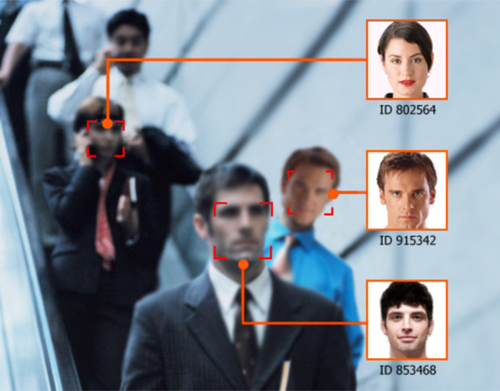
\includegraphics[width=0.75\linewidth]{figs/security.jpg}
\end{figure}
\end{frame}
%------------------------------------------------

\begin{frame}
\frametitle{Reconhecimento de Faces}
\begin{figure}
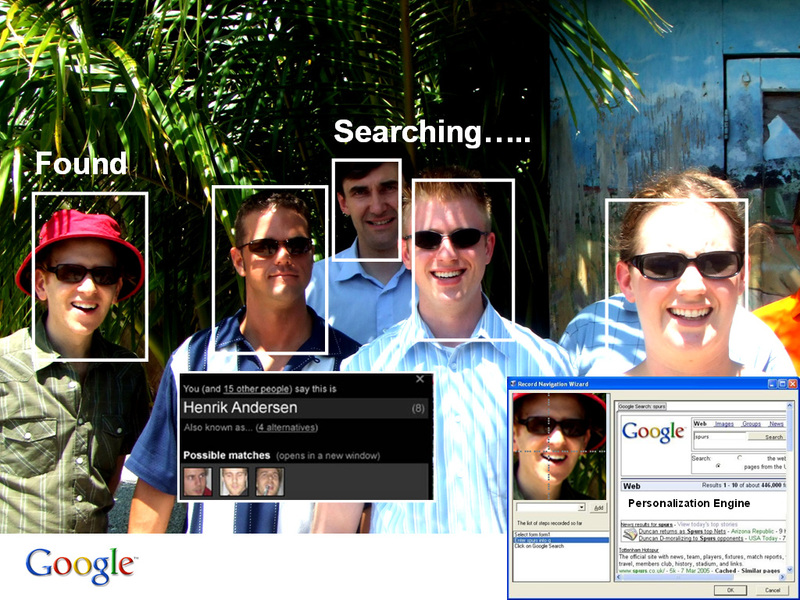
\includegraphics[width=0.75\linewidth]{figs/google.jpg}
\end{figure}
\end{frame}
%------------------------------------------------

\begin{frame}
\frametitle{Problemas}
\begin{itemize}
    \item As imagens de face pertencem a mesma pessoa?
    \item A face na imagem pertence a um indivíduo específico?
    \item O rosto pertence a alguma pessoa de um conjunto de indivíduos específicos?
\end{itemize}
\end{frame}
%------------------------------------------------
\subsection{Revisão de técnicas}
\begin{frame}
\frametitle{Eigenfaces ~\cite{eigenfaces}}
\begin{itemize}
    \item Redução de dimensionalidade de imagens de face.
    \item Reconhecimento se dá por medição de distância no espaço de \textit{eigenfaces}.
\end{itemize}
    \begin{figure}
    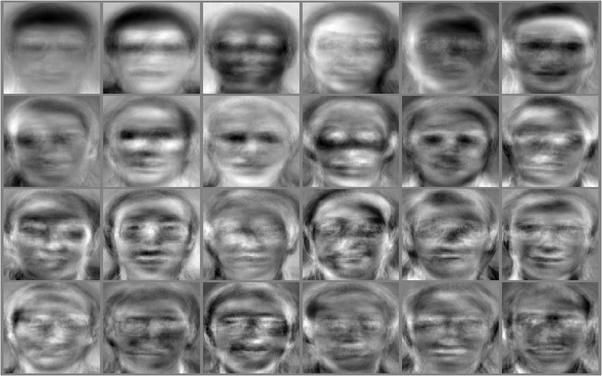
\includegraphics[width=0.75\linewidth]{figs/eigenfaces.png}
    \end{figure}
\end{frame}
%--------------------------------------------------
\begin{frame}
\frametitle{Deepface~\cite{deepface}}
\begin{itemize}
    \item Duas redes convolucionais profundas com pesos compartilhados.
    \item Modelo aprende a distanciar faces de pessoas diferentes.
\end{itemize}
    \begin{figure}
    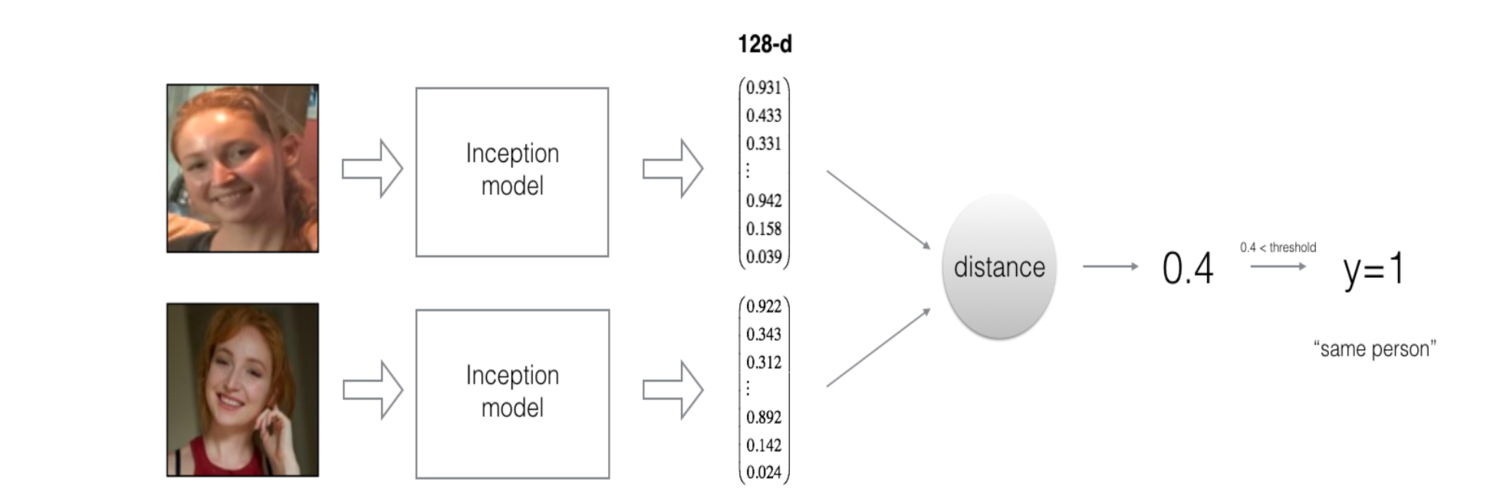
\includegraphics[width=\linewidth]{figs/siamese.png}
    \end{figure}
\end{frame}
%--------------------------------------------------
\begin{frame}
\frametitle{Facenet~\cite{facenet}}
\begin{itemize}
    \item Também aprende \textit{embedding} de face por rede neural profunda.
    \item Usa \textit{triplet loss}
\end{itemize}
    \begin{figure}
    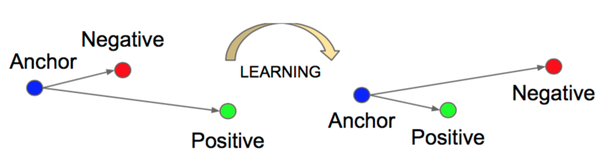
\includegraphics[width=0.75\linewidth]{figs/tripletLoss.png}
    \end{figure}
    \begin{equation}
        L=\sum_i^N\norm{f(x_i^a) - f(x_i^p)}_2^2 - \norm{f(x_i^a) - f(x_i^n)}_2^2 + \alpha
    \end{equation}
\end{frame}
%--------------------------------------------------
\subsection{Dataset}
\begin{frame}
\frametitle{Labeled faces in the wild~\cite{lfw}}
    \begin{itemize}
        \item 13233 imagens.
        \item 5749 indivíduos, 1680 com mais de uma imagem no conjunto.
        \item Rostos obtidos pelo Viola-Jones.
    \end{itemize}
    \begin{figure}
    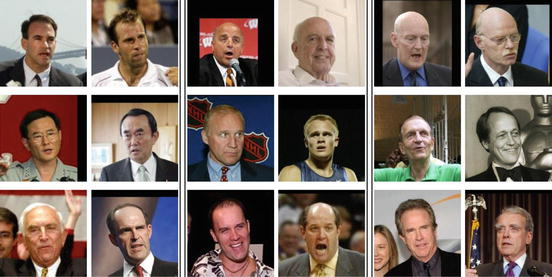
\includegraphics[width=0.75\linewidth]{figs/lfw.jpg}
    \end{figure}
\end{frame}
%--------------------------------------------------
\section{Extrator fixo}
\subsection{Modelo}
\begin{frame}
\frametitle{O modelo}
    \begin{itemize}
        \item Vetores de imagem computados por rede Xception treinada no ImageNet.
        \item Dois vetores de imagens são dados como entrada a uma camada completamente conectada com \textit{dropout} seguida de uma unidade sigmóide.
        \item Classifica se as imagens são da mesma pessoa ou não.
    \end{itemize}
    \begin{figure}
    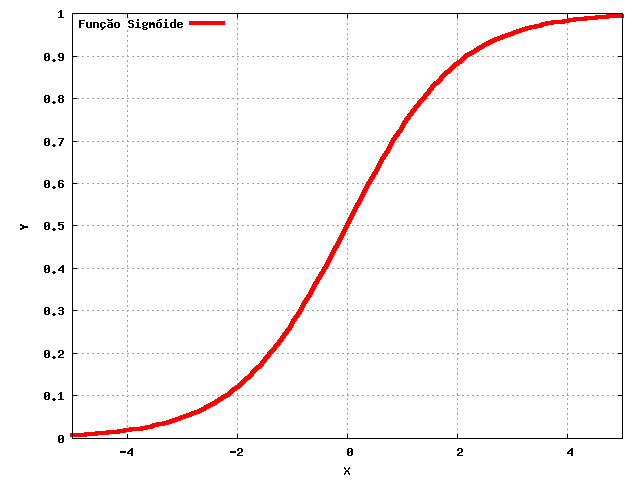
\includegraphics[width=0.5\linewidth]{figs/sigmoide.png}
    \end{figure}
\end{frame}
%--------------------------------------------------
\subsection{Experimentos}
\begin{frame}
\frametitle{Experimentos}
Hiperparâmetros:
\begin{itemize}
    \item Número de unidades:
        \begin{enumerate}
            \item 128
            \item 512
            \item 1024
        \end{enumerate}
    \item Probabilidade de dropout:
        \begin{enumerate}
            \item 0.2
            \item 0.5
            \item 0.8
        \end{enumerate}
    \item Modo de combinação de imagens:
        \begin{enumerate}
            \item Adição
            \item Concatenação
            \item Subtração
            \item Produto interno
            \item Produto elemento a elemento
        \end{enumerate}
\end{itemize}
\end{frame}
%--------------------------------------------------
\begin{frame}
\frametitle{Experimentos}
\begin{itemize}
    \item 2200 pares de treinamento.
    \item 1000 pares de validação.
    \item Minimização da entropia cruzada binária:
\end{itemize}
    \begin{equation}
    \textit{cross-entropy} = -{(y\log(p) + (1 - y)\log(1 - p))}\,.
    \end{equation}
\end{frame}
%------------------------------------------------------

\subsection{Resultados}
\begin{frame}
\frametitle{Resultados}
    Acurácia no treino e validação para diferentes valores de número de unidades e chance de dropout:
    
    \begin{figure}
    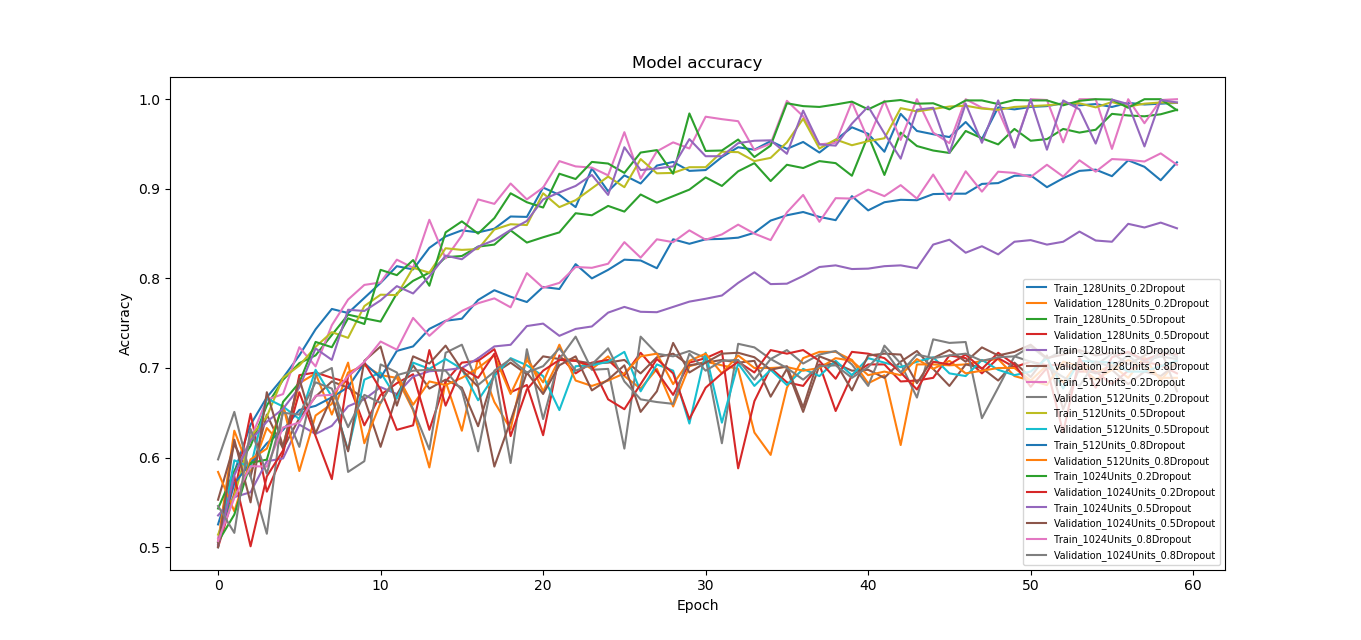
\includegraphics[width=\linewidth]{figs/curve.png}
    \end{figure}
\end{frame}

%------------------------------------------------------

\begin{frame}
\frametitle{Resultados}
    Resultados na primeira etapa de experimentos:
    
    \begin{table}
    \small
    \centering
    \begin{tabular}{|l|c|}
        \hline
        Modelo & Acurácia \\
        \hline
        Units\_128\_Drop\_0.2 & 0.718 \\
        Units\_128\_Drop\_0.5 & 0.721 \\
        Units\_128\_Drop\_0.8 & 0.719 \\
        Units\_512\_Drop\_0.2 & \textbf{0.735} \\
        Units\_512\_Drop\_0.5 & 0.718 \\
        Units\_512\_Drop\_0.8 & 0.726 \\
        Units\_1024\_Drop\_0.2 & 0.72 \\
        Units\_1024\_Drop\_0.5 & 0.728 \\
        Units\_1024\_Drop\_0.8 & 0.722 \\
        \hline
    \end{tabular}
\end{table}
\end{frame}

%------------------------------------------------------

\begin{frame}
\frametitle{Resultados}
    Acurácia no treino e validação para diferentes modos de combinação de entradas:
    
    \begin{figure}
    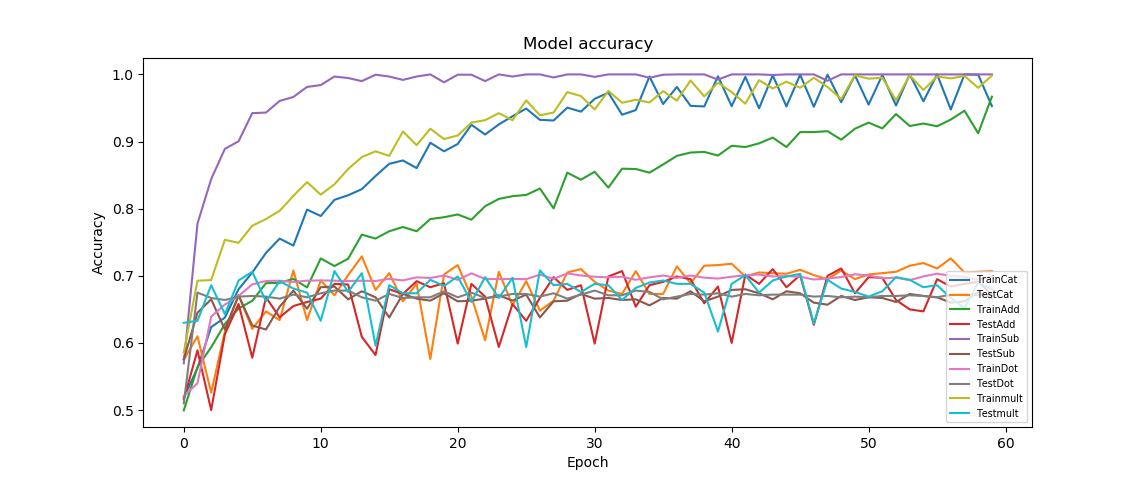
\includegraphics[width=\linewidth]{figs/curve_merge.png}
    \end{figure}
\end{frame}

%------------------------------------------------------

\begin{frame}
\frametitle{Resultados}
    Resultados na segunda etapa de experimentos:
    \begin{table}[htb]
    \small
    \centering
    \begin{tabular}{|l|c|}
        \hline
        Modelo & Acurácia \\
        \hline
        concat & \textbf{0.729} \\
        add & 0.711 \\
        subtract & 0.684 \\
        dotProduct & 0.678 \\
        multiply & 0.708 \\
        \hline

    \end{tabular}
\end{table}

\end{frame}

%------------------------------------------------------
\section{Pipeline de Detecção e Reconhecimento}
%------------------------------------------------------
\subsection{Datasets}
\begin{frame}
\frametitle{Datasets}
Dataset da turma:
\begin{itemize}
    \item 6 classes: Felipe, Lívia, Natália, Pedro, Rafael, Raphael e Unknown.
    \item Total de 36 imagens, sendo que todas as classes possuem 6 imagens, com exceção do Rafael (4 imagens) e Natália (2 imagens).
\end{itemize}  
O dataset LFW é o mesmo utilizado anteriormente, tirando o fato que é feito a detecção da face, antes do reconhecimento.
\end{frame}
%------------------------------------------------------
\begin{frame}
\subsection{Pipeline}
\frametitle{Pipeline}
\begin{tikzpicture}[node distance = 2.5cm, auto]
    % Place nodes
    \node [block] (input) {Input - dataset};
    \node [block, right of=input] (detect) {Detecta face};
    \node [block, right of=detect] (compute) {Computar as face embeddings de 128 dimensões};
    \node [block, right of=compute] (train) {Treina modelo nas embeddings computadas};
    %\node [block, left of=train] (recognize) {Reconhecer faces em imagens e video streams};
    \node [block, right of=train] (output) {Output - Modelo};
    
  	
    % Draw edges
    \path [line] (input) -- (detect);
    \path [line] (detect) -- (compute);
   	\path [line] (compute) -- (train);
    %\path [line] (train) -- (recognize);
    \path [line] (train) -- (output);
\end{tikzpicture}   
\end{frame}

%------------------------------------------------------

\begin{frame}
\frametitle{Detecção de Faces}
\begin{figure}
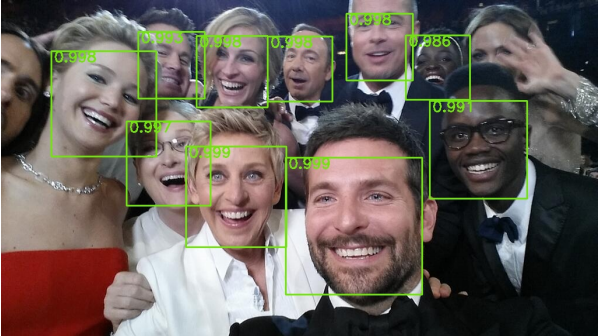
\includegraphics[width=0.95\linewidth]{figs/face_detection.png}
\end{figure}   
\end{frame}

%------------------------------------------------------

\begin{frame}
\frametitle{Cálculo das face embeddings}
\begin{figure}
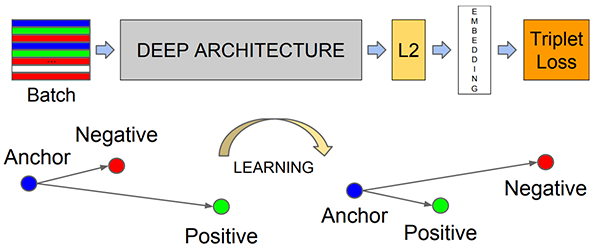
\includegraphics[width=1\linewidth]{figs/triplet_loss.png}
\end{figure}   
\end{frame}

%------------------------------------------------------
\begin{frame}
\frametitle{Treino do modelo}
\begin{figure}
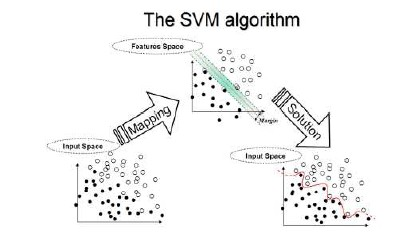
\includegraphics[width=1\linewidth]{figs/SvmFlow.jpg}
\end{figure}   
\end{frame}

%------------------------------------------------------
\begin{frame}
\subsection{Previsões e Resultados}
\frametitle{Previsão de novas imagens - Pipeline}
\begin{tikzpicture}[node distance = 3cm, auto]
    % Place nodes
    \node [block] (input) {Input - Imagem};
    \node [block, right of=input] (detect) {Detectar face};
    \node [block, right of=detect] (compute) {Computar as face embeddings de 128 dimensões};
    \node [block, below of=compute] (recognize) {Fazer classificação usando modelo salvo};
    \node [block, right of=recognize] (output) {Output - Imagem};
    
  	
    % Draw edges
    \path [line] (input) -- (detect);
    \path [line] (detect) -- (compute);
   	\path [line] (compute) -- (recognize);
    \path [line] (recognize) -- (output);
\end{tikzpicture}
\end{frame}
%------------------------------------------------------
\begin{frame}
\frametitle{Resultados}
\begin{figure}

\includegraphics[width=0.55\linewidth]{figs/Pedro_3.jpg}
\end{figure}   
\end{frame}
%------------------------------------------------------
\begin{frame}
\frametitle{Resultados}
\begin{figure}
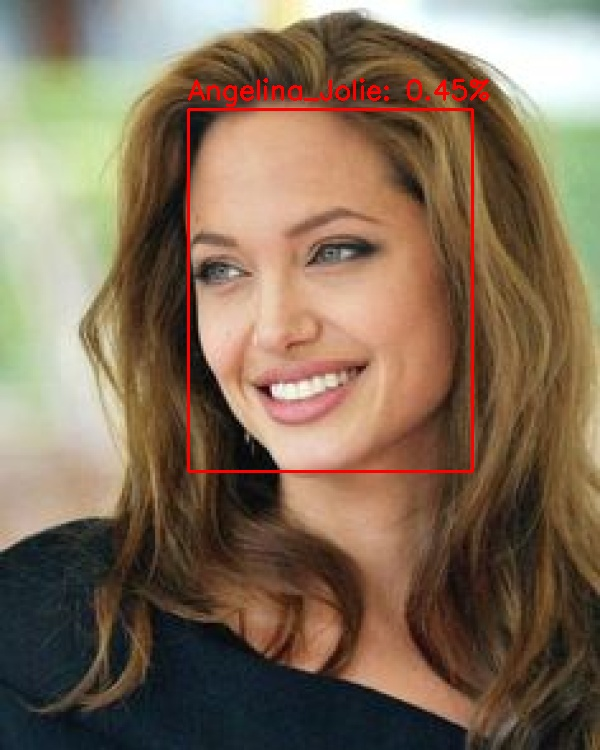
\includegraphics[width=0.50\linewidth]{figs/Angelina_Jolie_2.jpg}
\end{figure}   
\end{frame}
%------------------------------------------------------
\begin{frame}
\frametitle{Resultados}
\begin{figure}
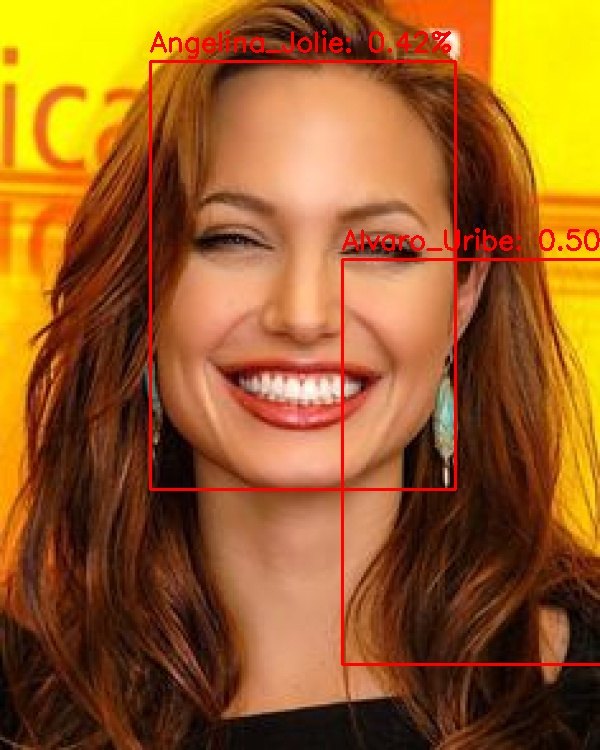
\includegraphics[width=0.50\linewidth]{figs/Angelina_Jolie_3.jpg}
\end{figure}   
\end{frame}
%------------------------------------------------------
\section{Conclusão}
\begin{frame}
\frametitle{Conclusão}
\begin{itemize}
    \item O modelo apresentado usando rede convolucional pré-treinada como extrator de características de imagens superou a baseline do conjunto de validação, alcançando 73.5\% de acurácia, contra os 50\% de baseline.
    \item Este modelo apresenta como vantagem grande rapidez de treinamento, simplicidade do modelo e desnecessidade de gerar característiscas manualmente.
    \item O pipeline construído para detecção e reconhecimento de faces mostrou-se muito bom para a detecção de faces nas imagens testadas, embora não tenha apresentado bons resultados para nenhum dos dois datasets abordados.
    \item Como trabalho futuro é interessante avaliar o último modelo tratado no mesmo dataset usado na parte 1.
\end{itemize}
\end{frame}

\begin{frame}[allowframebreaks]
\frametitle{References}
\footnotesize{
\begin{thebibliography}{99} % Beamer does not support BibTeX so references must be inserted manually as below
\bibitem[Turk e Pentland, 1991]{eigenfaces} Matthew A Turk e Alex P Pentland.
\newblock Face recognition using eigenfaces.
\newblock  In: IEEE Computer Society Conference on Computer Vision and Pattern Recognition, 1991, pages 586–591.

\bibitem[Taigman et al. 2014]{deepface} Yaniv Taigman, Ming Yang, Marc’Aurelio Ranzato, e Lior Wolf.
\newblock Deepface: Closingthe gap to human-level performance in face verification.
\newblock  In: IEEE Computer Society Conference on Computer Vision and Pattern Recognition, 2014.

\bibitem[Schroff et al. 2015]{facenet} lorian Schroff, Dmitry Kalenichenko, e James Philbin.
\newblock Facenet: A unified embed-ding for face recognition and clustering.
\newblock  In: IEEE Computer Society Conference on Computer Vision and Pattern Recognition, 2015.

\bibitem[Huan et al. 2008]{lfw} Gary B Huang, Marwan Mattar, Tamara Berg, e Eric Learned-Miller.  
\newblock Labeled faces in the wild: A database fo rstudying face recognition in unconstrained environments.
\newblock  In: Workshop on faces in ’Real-Life’ Images: detection, alignment, and recognition, 2008.

\end{thebibliography}
}
\end{frame}



\end{document}